\documentclass[xcolor={svgnames},
  hyperref={colorlinks},
  t,
  spanish, 12pt]{beamer}
\mode<presentation>

\usefonttheme[onlymath]{serif}
\setbeamertemplate{theorems}[ams style]
\usetheme{metropolis}
\useinnertheme{rectangles}
\usecolortheme{dolphin}

\setbeamercovered{highly dynamic}

\newcounter{saveenumi}
\newcommand{\seti}{\setcounter{saveenumi}{\value{enumi}}}
\newcommand{\conti}{\setcounter{enumi}{\value{saveenumi}}}

\resetcounteronoverlays{saveenumi}

\setbeamercolor{emph}{fg=purple}
\renewcommand<>{\emph}[1]{%

  {\usebeamercolor[fg]{emph}\only#2{\itshape}#1}%
}

\usepackage{fontenc}
\usepackage{graphicx}
\usepackage[utf8]{inputenc}
\usepackage[spanish,mexico]{babel}
\usepackage{fontenc}
\usepackage{amsmath}
\usepackage{amsthm}
\usepackage{amssymb}
\usepackage{graphicx}
\usepackage{mathrsfs}
\usepackage{yfonts}
\usepackage{enumerate}
\usepackage{mathtools}
\usepackage{textcomp}
\usepackage{lmodern}
\usepackage{fancyvrb}
\usepackage{multicol}
\usepackage{color}
\usepackage{verbatim}

\DefineVerbatimEnvironment{ColorVerbatim}{Verbatim}%
{formatcom=\color{purple},commandchars=\\\{\}}

\usepackage{etoolbox}

\BeforeBeginEnvironment{Verbatim}{\begingroup\color{purple}}%
\AfterEndEnvironment{Verbatim}{\endgroup}
\numberwithin{equation}{section}
\numberwithin{figure}{section}

\def\subsubsectionname{\translate{}}
\def\insertsubsubsectionnumber{\arabic{subsubsection}}
\setbeamertemplate{subsubsection page}
{
  \begin{centering}
    {\usebeamerfont{subsubsection name}\usebeamercolor[fg]{subsubsection
        name}\subsubsectionname}
    \vskip1em\par
    \begin{beamercolorbox}[sep=4pt,center]{part title}
      \usebeamerfont{subsubsection title}\insertsubsubsection\par
    \end{beamercolorbox}
  \end{centering}
}
\def\subsubsectionpage{\usebeamertemplate*{subsubsection page}}

\AtBeginSection{\frame{\sectionpage}}
\AtBeginSubsection{\frame{\subsectionpage}}
\AtBeginSubsubsection{\frame{\subsubsectionpage}}

\theoremstyle{plain}
  \newtheorem{thm}{Teorema}[section]
  \newtheorem{prop}{Proposici\'on}[section]
  \newtheorem{lem}[thm]{Lema}
  \newtheorem{cor}[thm]{Corolario}
  %\newtheorem{rem}{Observaci\'on}[chapter]
  \newtheorem*{sol}{Soluci\'on}
  \newtheorem{alg}{Algoritmo}[section]
  \newtheorem{solved}{Ejercicio Resuelto}
  \newtheorem{evc}{Evaluaci\'on Continua}

\theoremstyle{definition}
  \newtheorem{defn}{Definici\'on}[section]
  \newtheorem{conj}{Conjectura}[section]
  \newtheorem{exmp}{Ejemplo}[section]
  \newtheorem{exe}{Evaluaci\'on Continua}[section]
  \newtheorem{prob}{Problema}[section]
  \newtheorem{rem}{Observaci\'on}[section]
  \newtheorem*{ax}{Axioma}
  \newtheorem{tdv}{Tabla de Verdad}

\theoremstyle{remark}
  \newtheorem{claim}{Afirmaci\'on}[section]
  %\newtheorem{rem}{Observaci\'on}[chapter]
  %\newtheorem*{note}{Nota}
  \newtheorem{case}{Caso}
  \newtheorem{hint}{Sugerencia}[section]


\numberwithin{equation}{section}
\newcommand{\p}{\partial}
%\newcommand{\T}{\mathbb{T}}
\newcommand{\R}{\mathbb{R}}
\newcommand{\N}{\mathbb{N}}
\newcommand{\Q}{\mathbb{Q}}
\newcommand{\abs}[1]{\left|#1\right|}
\newcommand{\f}{\phi}
\newcommand{\vphi}{\varphi}
\newcommand{\vf}{\varphi}
\newcommand{\flow}[2]{\varphi^{#1}\left( #2 \right)}
\renewcommand{\d}[1]{\dot{#1}}
\renewcommand{\r}{\rho}
\newcommand{\A}{\mathcal{A}}
\newcommand{\gam}{\gamma}
\newcommand{\lam}{\lambda}
\renewcommand{\a}{\alpha}
\renewcommand{\b}{\beta}
\newcommand{\om}{\omega}
\newcommand{\iso}{\simeq}
\newcommand{\tensor}{\otimes}
\newcommand{\Z}{\mathbb{Z}}
\newcommand{\set}[1]{\left\{ #1 \right\}}
\newcommand{\inc}{\hookrightarrow}
\renewcommand{\L}{\mathcal{L}}
\renewcommand{\H}{\mathcal{H}}
\newcommand{\D}{\mathcal{D}}
\newcommand{\converge}[1]{\xrightarrow{#1}}
\renewcommand{\cot}{T^{*}}
\newcommand{\cott}[1]{T^{*}\T^{#1}}
\newcommand{\ep}{\epsilon}
\newcommand{\inp}[1]{\langle #1 \rangle}
%\newcommand{\G}{\mathcal{G}}
\newcommand{\hu}{\textbf{h}}
\newcommand{\deck}[1]{\operatorname{Dake}\left( #1 \right)}
\newcommand{\til}[1]{\tilde{#1}}
\newcommand{\Gam}{\Gamma}
\newcommand{\grad}{\nabla}
\newcommand{\del}{\delta}
\newcommand{\id}{\operatorname{Id}}
\newcommand{\Del}{\Delta}
\newcommand{\var}{\Delta}
\newcommand{\avch}[2]{\frac{\Delta #1}{\Delta #2}}
\newcommand{\Avch}[2]{\dfrac{\Delta #1}{\Delta #2}}
\newcommand{\Err}{\operatorname{Err}}
\newcommand{\imply}{\rightarrow}
\newcommand{\wed}{\wedge}
\newcommand{\biconditional}{\longleftrightarrow}
\newcommand{\yields}{\vdash}
\newcommand{\onlyif}{\Rightarrow}
\newcommand{\uset}{\mathbb{U}}
\newcommand{\minus}{\backslash}
\newcommand{\symdif}{\oplus}
\newcommand{\rel}[1]{\boxed{{\color{blue}\textbf{#1}}}}
\newcommand{\dom}[1]{\operatorname{Dom}\left( #1 \right)}
\newcommand{\im}[1]{\operatorname{Im}\left( #1 \right)}
\newcommand{\nrel}[1]{\boxed{{\color{red}\not}{\color{orange}\textbf{#1}}}}
\newcommand{\comp}[2]{#1 \circ #2}

%\date{\today}
\title{Matemáticas Discretas \\
  Teoría de Gráficas}
\author[Juliho Castillo]{Dr. Juliho Castillo}

\date{\today}

\begin{document}

\frame{
  \titlepage
}

\begin{frame}[allowframebreaks=0.5]
  \tableofcontents
\end{frame}

\section{Matrices}

\begin{frame}
  Las matrices son arreglos rectangulares de número que nos ayudan a codificar
  información. Por ejemplo:
  $$
    \begin{pmatrix}
      a_{1,1} & a_{1,2} \\
      a_{2,1} & a_{2,2}
    \end{pmatrix}
  $$
  puede ser útil para codificar los coeficientes del sistema de ecuaciones:
  $$
    \begin{cases}
      a_{1,1}x+a_{1,2}y=b_{1} \\
      a_{2,1}x+a_{2,2}y=b_{2}
    \end{cases}
  $$
\end{frame}

\begin{frame}
  En general, una matriz tiene la forma
  \begin{equation}
    \label{A}
    \tag{A}
    \begin{pmatrix}
      a_{1,1} & a_{1,2} & \cdots & a_{1,n} \\
      \vdots  &         &        & \vdots  \\
      a_{m,1} & a_{m,2} & \cdots & a_{m,n}
    \end{pmatrix}
  \end{equation} \pause

  Los subíndices de cada elemento $a_{i,j}$ denotan la posición del mismo:
  $i$ es el número del \emph{renglón} (contando de arriba a abajo), mientras
  que $j$ es el número de la columna (contanto de izquierda a derecha).
\end{frame}

\begin{frame}
  Podemos extraer renglones y columnas de la matrix \eqref{A}: El $i-$esímo
  renglón es
  $$
    R_{i}=
    \begin{pmatrix}
      a_{i,1} & \cdots & a_{i,n}
    \end{pmatrix}
  $$ \pause
  mientras que la $j-$ésima columna será
  $$
    C_{j}=
    \begin{pmatrix}
      a_{j,1} \\
      \vdots  \\
      a_{j,m}
    \end{pmatrix}
  $$
\end{frame}

\begin{frame}
  Diremos que la matriz \eqref{A} tiene dimensión $m\times n.$ \pause

  Si existe un conjunto de números $F,$ tal que todos los elementos $a_{i,j}$
  de la matriz pertenecen a dicho conjunto, diremos que la matriz tiene
  coeficientes en $F.$ \pause
\end{frame}

\begin{frame}
  \begin{rem}
    Para que las operaciones entre matrices estén bien definidas, es necesario
    que la suma, resta y multiplicación entre entre elementos de $F$ también
    este bien definida. Por esto generalmente $F$ se elige como $\R$ o $\Z.$
  \end{rem}
\end{frame}

\begin{frame}
  La colección de todas las matrices de dimensión $m\times n$ con
  coeficientes en $F$ se denotará por $$M_{m,n}(F).$$
\end{frame}

\begin{frame}
  \begin{defn}
    Las matrices de dimensión $m\times 1$ se conocen como \emph{vectores
      columna,} mientras que las de dimensión $1\times n$ se conocen como
    \emph{vectores renglón.}
    \pause

    La colección $M_{m,1}(F)$ de todos los vectores columna con coeficientes
    comunmente se denota por $F^{m}.$ \pause Mientras que la colección
    $M_{1,n}(F)$ de todos los vectores columna con coeficientes  comunmente se
    denota por $F^{n\ast}.$

  \end{defn}
\end{frame}

\subsection{Operaciones elementales}

\begin{frame}
  Por brevedad, la matriz \eqref{A} se denota por $A=[a_{i,j}].$ \pause

  En el caso de los vectores renglones y columnas, podemos omitir el subíndice
  fijo
  $$R=[R_{1,j}]=[R_{j}], \; C=[C_{i,1}]=[C_{i}].$$
\end{frame}

\begin{frame}
  Si $B=[b_{i,j}]$ es otra matriz de dimensión $m\times n,$ la suma se define
  como $$A+B=[a_{i.j}+b_{i,j}].$$\pause

  De manera similar, la resta se define como $$A-B=[a_{i,j}-b_{i,j}].$$
\end{frame}

\begin{frame}
  \begin{exmp}
    $$
      \begin{pmatrix}
        1 & -1 & 0  \\
        2 & 3  & -4
      \end{pmatrix}
      +
      \begin{pmatrix}
        7 & 0  & -1 \\
        2 & -1 & 5
      \end{pmatrix} =
    $$ \pause
    $$
      \begin{pmatrix}
        1 & -1 & 0  \\
        2 & 3  & -4
      \end{pmatrix}
      -
      \begin{pmatrix}
        7 & 0  & -1 \\
        2 & -1 & 5
      \end{pmatrix} =
    $$
  \end{exmp}

\end{frame}

\begin{frame}
  Observe que para que la \emph{suma y resta} tenga sentido, ambas matrices deben
  tener exactamente las \emph{mismas dimensiones}. \pause

  Después de ver la facilidad para definir la suma y resta, uno se ve tentado a
  definir la multiplicación de la misma forma. Pero tal definición es poco
  útil en las aplicaciones. \pause

  Por esta razón, desarrollaremos el concepto de multiplicación, a fin de
  poder aplicar esta operación en la resolución de problemas.
\end{frame}

\subsection{Multiplicación}
\begin{frame}
  \begin{defn}
    Sean $R=[R_{j}]$ un vector renglón y $C=[C_{i}]$ un vector columna, ambos de
    longitud $n.$
    \pause
    El \emph{producto renglón-columna} se define como
    \begin{equation}
      \label{RC}
      \tag{RC}
      RC=
      \begin{pmatrix}
        R_{1} & \cdots & R_{n}
      \end{pmatrix}
      \begin{pmatrix}
        C_{1} \\ \vdots \\ C_{n}
      \end{pmatrix}
      =
      \sum_{i=1}^{n} R_{j}C_{i}.
    \end{equation}

  \end{defn}

\end{frame}

\begin{frame}
  \begin{exmp}
    Considere
    $$
      R=
      \begin{pmatrix}
        1 & 0 & -1
      \end{pmatrix}, \;
      C=
      \begin{pmatrix}
        2 \\ 1 \\ -2
      \end{pmatrix}.
    $$

    Calcule $RC.$

  \end{exmp}

\end{frame}

\begin{frame}
  \begin{exmp}
    Reescriba la siguiente ecuación, utilizando el \emph{producto
      renglón-columna}:
    $$2x-3y+z=0.$$
  \end{exmp}

\end{frame}

\begin{frame}
  \begin{defn}
    Sea $A=[a_{i,j}]\in M_{m\times n}$ y $B=[b_{j,k}]\in M_{n\times l}.$ Definimos
    su producto como
    \begin{equation}
      \label{AB}
      \tag{AB}
      AB=
      \begin{pmatrix}
        R_{i}C_{k}
      \end{pmatrix}
    \end{equation}
    donde $R_{i}$ es el $i-$ésimo renglón de $A$ y $C_{k}$ es la $k-$ésima
    columna de $B.$
  \end{defn}

\end{frame}

\begin{frame}
  \begin{rem}
    \begin{itemize}
      \item Para que esta multiplicación tenga sentido, los renglones de $A$ y
            las columnas de $B$ deberán tener la misma longitud $n.$
            \pause
      \item La matriz resultante tendrá dimensión $m \times l.$ \pause
      \item A menos que $m=l,$ el producto $BA$ podría no estar definido. \pause
      \item Aun cuando $BA$ estuviera bien definido, el producto de matrices no es
            \emph{conmutativo,} es decir, generalmente tendremos que $$AB \neq BA.$$
    \end{itemize}
  \end{rem}

\end{frame}

\begin{frame}
  \begin{exmp}
    Encuentre el producto $AB$ de las siguientes matrices
    $$A= \left(\begin{array}{r}
        0
      \end{array}\right) $$
    $$B= \left(\begin{array}{rr}
        0 & -1
      \end{array}\right) $$
    \pause Solución:
    $$AB= \left(\begin{array}{rr}
        0 & 0
      \end{array}\right) $$
  \end{exmp}
\end{frame}

\begin{frame}
  \begin{exmp}
    Encuentre el producto $AB$ de las siguientes matrices
    $$A= \left(\begin{array}{rr}
        0  & -1 \\
        -1 & 0  \\
        0  & 0
      \end{array}\right) $$
    $$B= \left(\begin{array}{rrr}
        0 & -1 & 0 \\
        0 & 0  & 0
      \end{array}\right) $$
    \pause Solución:
    $$AB= \left(\begin{array}{rrr}
        0 & 0 & 0 \\
        0 & 1 & 0 \\
        0 & 0 & 0
      \end{array}\right) $$
  \end{exmp}
\end{frame}

\begin{frame}
  \begin{exmp}
    Encuentre el producto $AB$ de las siguientes matrices
    $$A= \left(\begin{array}{r}
        -1 \\
        -1 \\
        0
      \end{array}\right) $$
    $$B= \left(\begin{array}{rrr}
        -1 & 0 & 0
      \end{array}\right) $$
    \pause Solución:
    $$AB= \left(\begin{array}{rrr}
        1 & 0 & 0 \\
        1 & 0 & 0 \\
        0 & 0 & 0
      \end{array}\right) $$
  \end{exmp}
\end{frame}

\begin{frame}
  \begin{exmp}
    Encuentre el producto $AB$ de las siguientes matrices
    $$A= \left(\begin{array}{r}
        6  \\
        -9 \\
        -10
      \end{array}\right) $$
    $$B= \left(\begin{array}{r}
        -5
      \end{array}\right) $$
    \pause Solución:
    $$AB= \left(\begin{array}{r}
        -30 \\
        45  \\
        50
      \end{array}\right) $$
  \end{exmp}
\end{frame}

\begin{frame}
  \begin{exmp}
    Encuentre el producto $AB$ de las siguientes matrices
    $$A= \left(\begin{array}{r}
        2
      \end{array}\right) $$
    $$B= \left(\begin{array}{rrr}
        -1 & 1 & -3
      \end{array}\right) $$
    \pause Solución:
    $$AB= \left(\begin{array}{rrr}
        -2 & 2 & -6
      \end{array}\right) $$
  \end{exmp}
\end{frame}

\begin{frame}
  \begin{exmp}
    Encuentre el producto $AB$ de las siguientes matrices
    $$A= \left(\begin{array}{rr}
        -1 & -3 \\
        -7 & -1
      \end{array}\right) $$
    $$B= \left(\begin{array}{r}
        -7 \\
        -4
      \end{array}\right) $$
    \pause Solución:
    $$AB= \left(\begin{array}{r}
        19 \\
        53
      \end{array}\right) $$
  \end{exmp}
\end{frame}

\begin{frame}
  \begin{exmp}
    Rescriba el siguiente sistema de ecuación en forma matricial y encuentre su
    solución:
    $$
      \begin{cases}
        -x-3y=19 \\
        -7x-y=53
      \end{cases}
    $$
  \end{exmp}

\end{frame}

\section{Teoría general de grafos}

\begin{frame}
  En matemáticas, la \emph{teoría de grafos} estudia estructuras
  matemáticas usadas para modelar relaciones por pares entre objetos.
\end{frame}

\subsection{Definición de grafo}

\begin{frame}{Concepto de gráfo}
  Un \emph{grafo} $G$ consiste de:
  \begin{enumerate}[(a)]
    \item Un conjunto $V$ cuyos elementos son llamados \emph{vértices,} puntos o
          nodos de $G.$
    \item Un conjunto $E$ de pares (no ordenados) de distintos vertices, a los que
          llamaremos \emph{aristas} de $G.$
  \end{enumerate}

  Denotaremos un grafo por $G(V,E)$ cuando querramos enfatizar los componentes
  del mismo.
\end{frame}

\begin{frame}
  \begin{rem}
    Debido a una ambig\"uedad en la traducción del inglés al espa\~nol, en
    ocasiones, a un grafo también se le conoce como \emph{gráfica,} que se
    puede confundir con el concepto de teoría de conjuntos. En este material, a
    veces utilizaremos \textit{gráfica,} pero debe entenderse como un grafo.
  \end{rem}
\end{frame}

\begin{frame}
  \begin{figure}[h!]
    \centering
    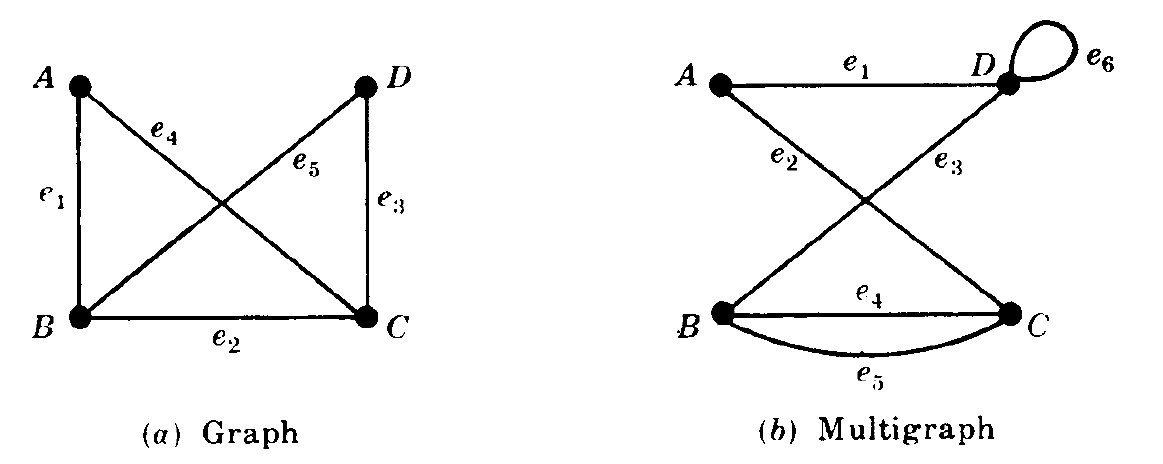
\includegraphics[width=12cm,keepaspectratio=true]{./grafos.png}
    % grafos.png: 0x0 pixel, 300dpi, 0.00x0.00 cm, bb=
    \caption{Grafos y multigrafos}
    \label{fig:md0501}
  \end{figure}

\end{frame}

\begin{frame}{Multigrafos}
  Consideremos la figura \ref{fig:md0501} (b). Las aristas $e_{4}$y $e_{5}$ son
  llamadas \emph{aristas multiples} ya que conectan los mismos extremos, \pause
  mientras que la arista $e_{6}$ es llamada \emph{bucle} ya que conecta un
  vértice consigo mismo.

\end{frame}

\begin{frame}
  Tales diagramas son llamados \emph{multigrafos;} \pause la definición formal
  de grafo no admite aristas multiples ni bucles.
\end{frame}

\begin{frame}
  \begin{rem}
    Sin embargo, algunos textos utilizan ``grafos'' para referirse a lo que
    nosotros llamaremos multigrafos, mientras que ocupan ``grafo simple'' para lo
    que nosotros llamaremos grafos.
  \end{rem}

\end{frame}

\begin{frame}{Grado de un vértice}
  El \emph{grado} de un vértice $v$ es un grafo $G,$ denotado por $\deg(v),$ es
  igual al número de aristas in $G$ que contienen a $v,$ es decir, que
  \emph{inciden} en $v.$
\end{frame}

\begin{frame}
  Dado que cada arista incide en dos vértices diferentes, tenemos el siguiente
  resultado simple pero importante:
  \begin{thm}
    La suma de los grados de los vértices en un grafo $G$ es el doble del
    número de aristas.
  \end{thm}

\end{frame}

\begin{frame}
  \begin{exmp}
    En el grafo de la figura \ref{fig:md0501}(a), tenemos que
    $$\deg(A)=2, \; \deg(B)=3,\; \deg(C)=3, \; \deg(D)=2.$$
    \pause

    La suma de los grados es igual a 10, que es dos veces el número de aristas.
  \end{exmp}

\end{frame}

\begin{frame}
  \begin{defn}
    Diremos que un vértice es \emph{par} o \emph{impar} de acuerdo a la paridad
    de su grado.
    \pause
    En el ejemplo anterior, tanto $A$ com $D$ son vértices pares, mientras que
    $B$ y $C$ son impares.
  \end{defn}

\end{frame}

\begin{frame}
  \begin{rem}
    Diremos que un vertice de grado cero está \emph{aislado.}
  \end{rem}
\end{frame}

\begin{frame}{Gráfos finitos y triviales}
  Diremos que un grafo  es \emph{finito} si tiene un número finito de
  vértices y un número finito de aristas. \pause

  Observe que un número finito de vértices implica un número finito de
  aristas; pero no lo contrario no es necesariamente cierto. \pause

  Diremos que un grafo con un único vértice, sin aristas,  es
  \emph{trivial.}\
\end{frame}

\begin{frame}
  \begin{rem}
    A menos que se indique de otra manera, sólo trataremos con grafos finitos.
  \end{rem}

\end{frame}

\subsection{Subgrafos y grafos homeomorfos e isomorfos}

\begin{frame}
  Ahora, discutiremos relaciones de equivalencia entre grafos.
\end{frame}

\begin{frame}{Subgrafos}
  Consideremos un grafo $G(V,E).$ Diremos que otro grafo $H(V',E')$ es un
  \emph{subgrafo} de $G$ si los vértices y aristas de $H$ están contenidos en
  los vértices y aristas de $G,$ es decir,
  $$
    V'\subset V, \; E' \subset E.
  $$
\end{frame}

\begin{frame}
  En particular:
  \begin{enumerate}[(a)]
    \item Un subgrafo $H(V',E')$ de $G(V,E)$ es llamado subgrafo \emph{inducido}
          por sus vértices $V'$ si el conjunto de aristas $E'$ contiene todas las
          aristas en $G$ cuyo extremos pertenecen a los vértices en $H.$ \pause
    \item Si $v$ es un vértice en $G,$ entonces \emph{$G-v$} es el subgrafo de
          $G$ ontenido al borrar $v$ de $G$ y todas las aristas en $G$ que inciden en
          $v.$ \pause
    \item Si $e$ es una arista en $G,$ entonces \emph{$G-e$} es el subgrafo de $G$
          obtenido borrando la arista $e$ en $G.$
  \end{enumerate}

\end{frame}

\begin{frame}{Grafos isomorfos}
  Dos grafos $G(V,E)$ y $G^{*}(V^{*},E^{*})$ son llamados \emph{isomorfos} si
  existe una función biyectiva $f: V \to V^{*}$ tal que: $\set{u,v}$ es una
  arista de $G$ si y solo si $\set{f(u),f(v)}$ es una arista de $G^{*}.$
  \pause

  La idea es que estos grafos son equivalentes, aún cuando sus representaciones
  pueden lucir muy diferentes.
\end{frame}

\begin{frame}
  \begin{figure}[h!]
    \centering
    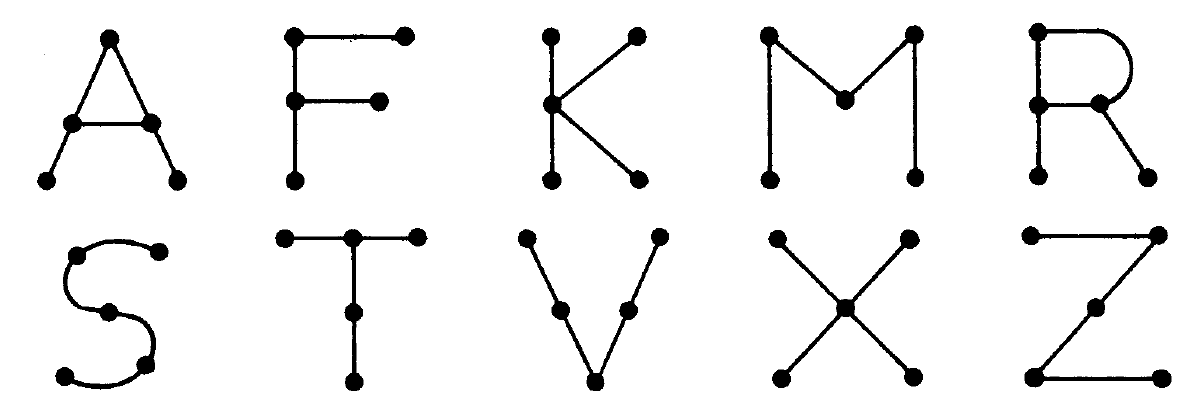
\includegraphics[width=10cm,keepaspectratio=true]{./letras.png}
    % letras.png: 0x0 pixel, 300dpi, 0.00x0.00 cm, bb=
    \caption{Grafos isomorfos.}
    \label{fig:md0502}
  \end{figure}

\end{frame}

\begin{frame}{Grafos homeomorfos}
  Dado un grafo $G,$ podemos obtener un nuevo grafo dividiendo una arista de $G$
  con vértices adicionales. \pause

  Dos grafos $G$ y $G^{*}$ son llamados \emph{homeomorfos} si pueden obtenerse de
  gráficas isomorfas a través de este método.
\end{frame}

\begin{frame}
  \begin{figure}[h!]
    \centering
    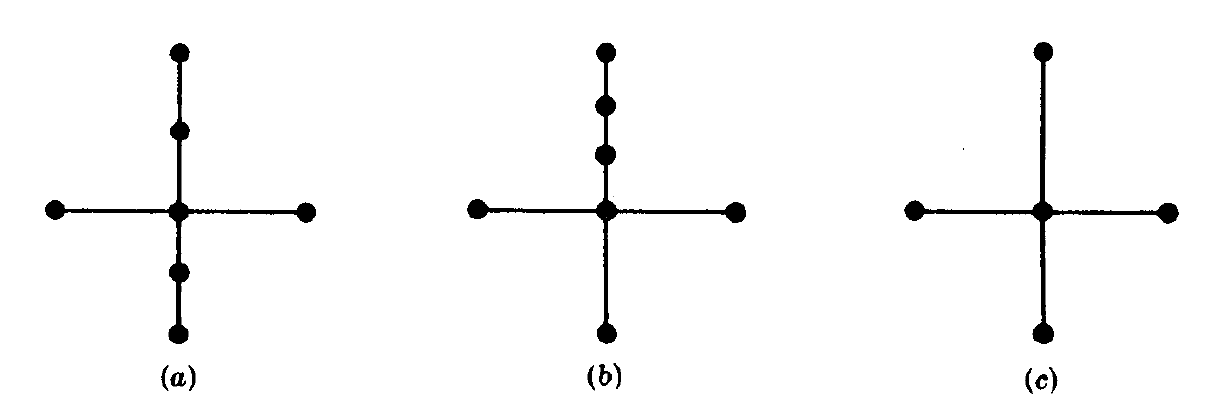
\includegraphics[width=8cm,keepaspectratio=true]{./homomorfas.png}
    % homomorfas.png: 0x0 pixel, 300dpi, 0.00x0.00 cm, bb=
    \caption{Grafos homomorfos}
    \label{fig:md0503}
  \end{figure}

  Los grafos $(a)$ y $(b)$ son homeomorfos, ya que se pueden obtener a\~nadiendo
  vértices al grafo $(c).$
\end{frame}

\subsection{Caminos y conexidad}

\begin{frame}
  Un \emph{camino} en un (multi)grafo $G$ consiste en una sucesión alternante
  de vértices y arista de la forma
  $$
    v_{0}, e_{1}, v_{1}, ..., e_{n-1}, v_{n-1}, e_{n}, v_{n}
  $$
  donde cada arista $e_{i}$ contiene los vértices $v_{i-1}$ y $v_{i}.$
\end{frame}

\begin{frame}
  \begin{rem}
    Observe que en grafo, podemos simplificar la notación para un camino,
    indicando sólo los vértices que recorre:
    $$v_{0}, v_{1},..., v_{n}.$$
  \end{rem}
\end{frame}

\begin{frame}
  Diremos que el camino es \emph{cerrado} si $v_{n}=v_{0}.$ En otro caso, diremos
  que el camino conecta $v_{0}$ con $v_{n}.$
  \pause

  Un \emph{camino simple} es aquel en el cual todos los vértices son distintos.
  Mientras que un camino en el que todas las aristas son distintas se llama
  \emph{paseo}.
  \pause
\end{frame}

\begin{frame}
  La \emph{longitud} de un camino es igual a número de aristas en la sucesión
  que lo define.
  \pause
\end{frame}

\begin{frame}
  Un \emph{ciclo} es un camino cerrado de \emph{longitud} al menos 3, en el que
  todos los vértices son distintos, excepto el inicial $v_{0}$ y el final
  $v_{n}.$
  \pause

  Un ciclo de longitud $k$ es llamado \emph{$k-$ciclo.}
\end{frame}

\begin{frame}
  \begin{figure}[h!]
    \centering
    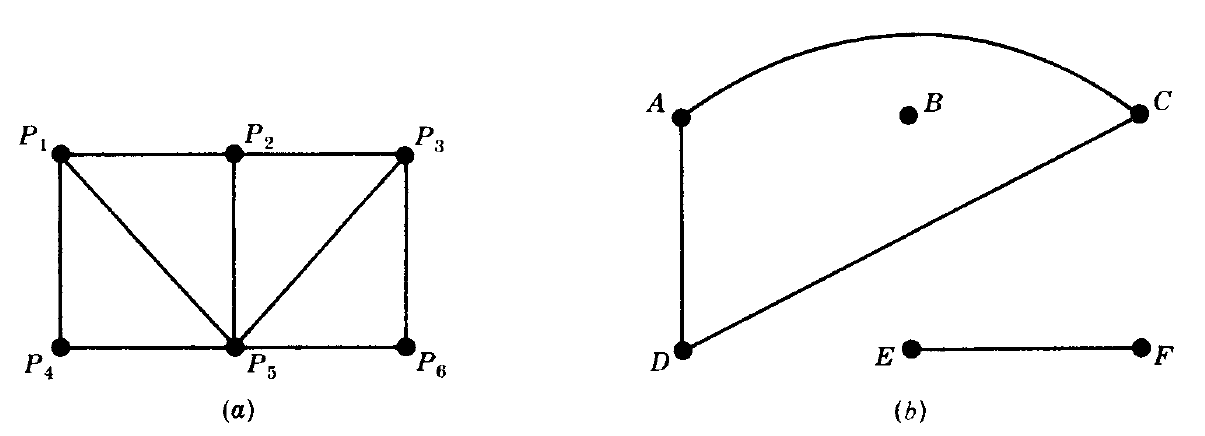
\includegraphics[width=10 cm,keepaspectratio=true]{./grafo_8_8.png}
    % grafo_8.8.png: 0x0 pixel, 300dpi, 0.00x0.00 cm, bb=
    \caption{Conexidad en grafos}
    \label{fig:md0504}
  \end{figure}
\end{frame}

\begin{frame}
  \begin{exmp}
    \label{lip:exmp:8.1}
    Consideremos el grafo \ref{fig:md0504}(a). Considere las siguientes sucesiones
    \begin{align*}
      \a   & =\left( P_{4}, P_{1}, P_{2}, P_{5}, P_{1},P_{2}, P_{3}, P_{6}  \right), \\
      \b   & =\left( P_{4}, P_{1}, P_{5}, P_{2}, P_{6} \right)                       \\
      \gam & = \left( P_{4}, P_{1}, P_{5}, P_{2}, P_{3}, P_{5}, P_{6} \right)        \\
      \del & =\left( P_{4}, P_{1}, P_{5}, P_{3}, P_{6} \right).
    \end{align*}

  \end{exmp}

\end{frame}

\begin{frame}
  \begin{figure}[h!]
    \centering
    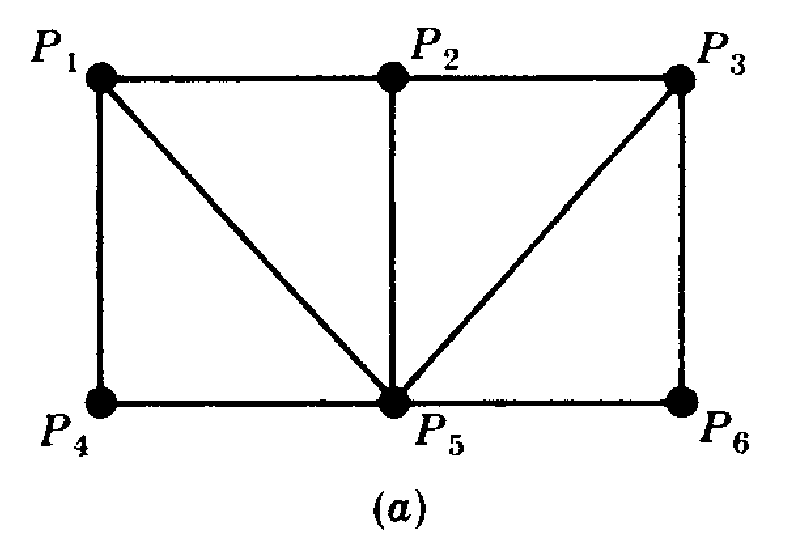
\includegraphics[width=5cm,keepaspectratio=true]{./grafo_8_8_a.png}
    % grafo_8_8_a.png: 0x0 pixel, 300dpi, 0.00x0.00 cm, bb=
  \end{figure}
  $\a$ es un camino de $P_{4}$ a $P_{6},$ pero no es un paseo.
\end{frame}

\begin{frame}
  \begin{figure}[h!]
    \centering
    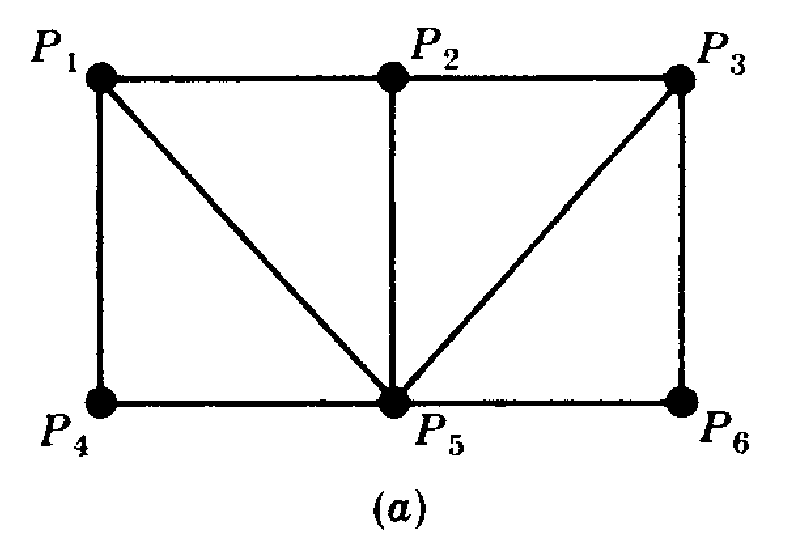
\includegraphics[width=5cm,keepaspectratio=true]{./grafo_8_8_a.png}
    % grafo_8_8_a.png: 0x0 pixel, 300dpi, 0.00x0.00 cm, bb=
  \end{figure}
  $\b$ no es un camino, ya que no existe alguna arista $\set{P_{2}, P_{6}}.$
\end{frame}

\begin{frame}
  \begin{figure}[h!]
    \centering
    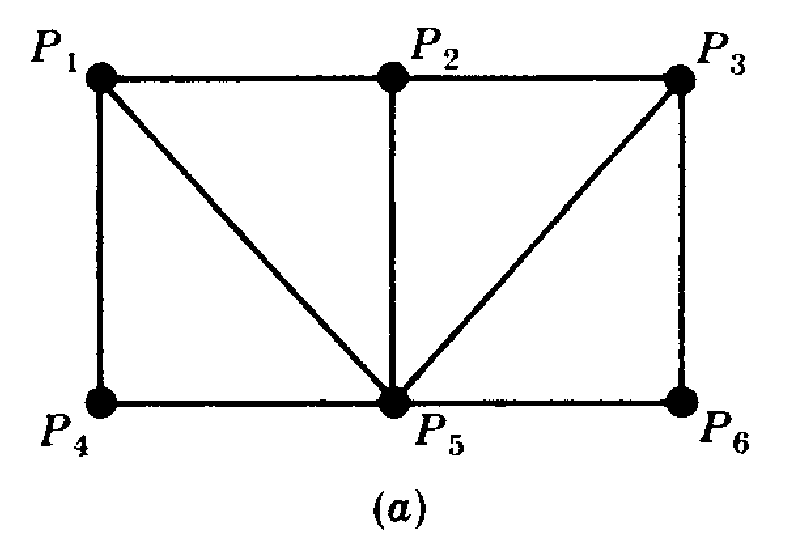
\includegraphics[width=5cm,keepaspectratio=true]{./grafo_8_8_a.png}
    % grafo_8_8_a.png: 0x0 pixel, 300dpi, 0.00x0.00 cm, bb=
  \end{figure}
  $\gam$ es un paseo, pero no es un camino simple.
\end{frame}

\begin{frame}
  \begin{figure}[h!]
    \centering
    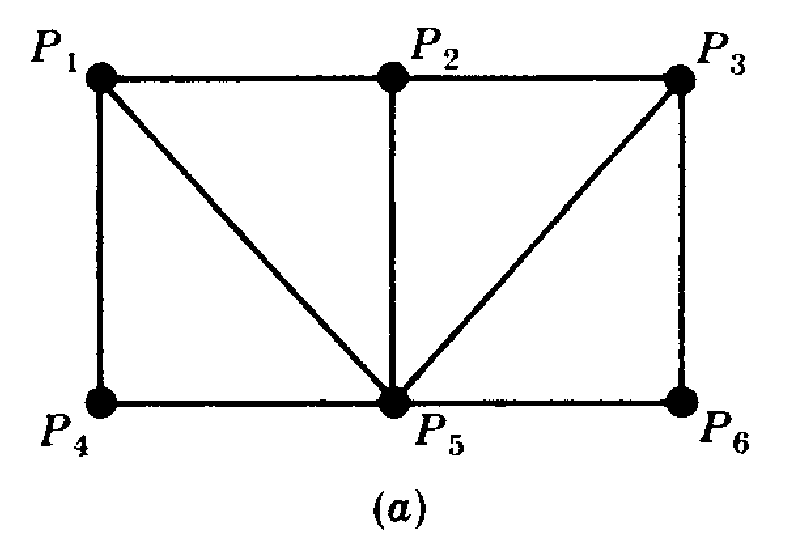
\includegraphics[width=5cm,keepaspectratio=true]{./grafo_8_8_a.png}
    % grafo_8_8_a.png: 0x0 pixel, 300dpi, 0.00x0.00 cm, bb=
  \end{figure}
  $\del$ es un camino simple de $P_{4}$ a $P_{6},$ pero no es el camino más
  corto, es decir, con el meno número de aristas. ?`Cuál es el camino más
  corto?
\end{frame}

\begin{frame}
  Eliminando aristas innecesarias, no es difícil ver que cualquier camino de
  $u$ a $v$ puede ser reemplazado por un camino simple.
  \pause

  Formalmente:
  \begin{thm}
    Existe un camino del vértice $u$ a $v$ si y solo si existe un camino simple
    de $u$ a $v.$
  \end{thm}

\end{frame}

\begin{frame}{Conexidad y componentes conexas}
  Un grafo $G$ es conexo si existe un camino entre cualesquiera dos vértices.
  \pause Por ejemplo, el grafo \ref{fig:md0504}(a) es conexo, pero no así el
  grafo \ref{fig:md0504}(b).
  \begin{figure}[h!]
    \centering
    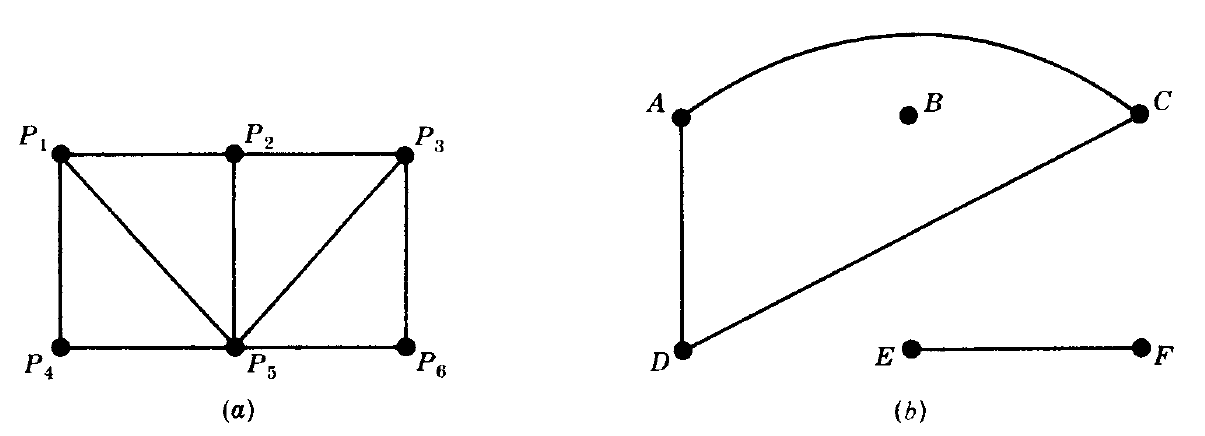
\includegraphics[width=8cm,keepaspectratio=true]{./grafo_8_8.png}
    % grafo_8_8.png: 0x0 pixel, 300dpi, 0.00x0.00 cm, bb=
  \end{figure}

\end{frame}

\begin{frame}
  Consideremos un grafo $G.$ Un subgrafo conexo $H$ de $G$ es llamado
  \emph{componente conexa} de $G$ si $H$ no está contenido de manera propia en
  cualquier otro grafo conexo de $G.$\pause

  Por ejemplo, el grafo \ref{fig:md0504}(b) tiene tres componentes conexas.

  \begin{figure}[h!]
    \centering
    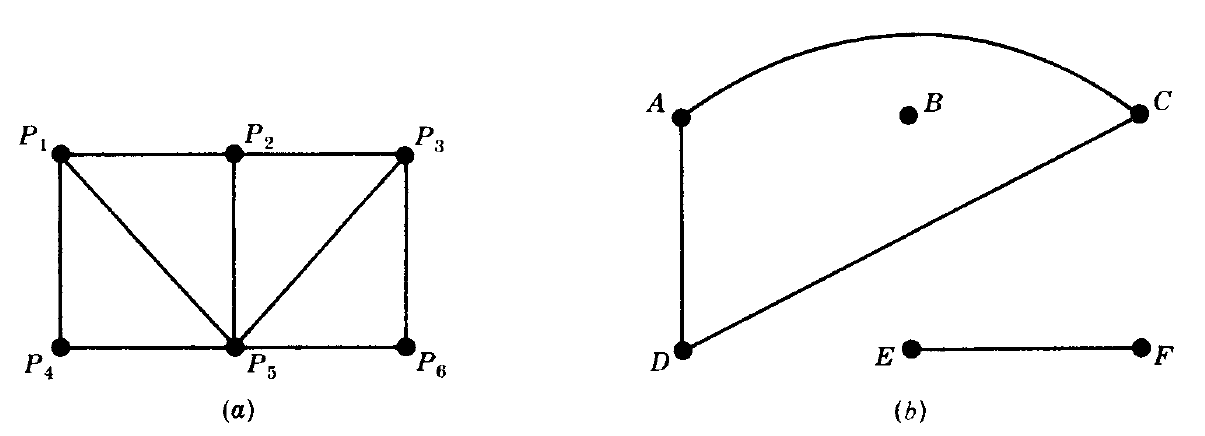
\includegraphics[width=8cm,keepaspectratio=true]{./grafo_8_8.png}
    % grafo_8_8_a.png: 0x0 pixel, 300dpi, 0.00x0.00 cm, bb=
  \end{figure}

\end{frame}

\begin{frame}
  \begin{rem}
    Formalmente, permitiendo que un vértice $u$ esté conectado consigo mismo,
    la relación \begin{center}
      \texttt{$u$ está conectado con $v$}

    \end{center}
    es una relación de equivalencia en el conjunto de vértices del grafo $G,$
    \pause y las clases de equivalencia de esta relación son las componentes
    conexas de $G.$
  \end{rem}

\end{frame}

\begin{frame}{Distancia y diametro}
  Consideremos un grafo conexo $G.$ La distancia entre  dos vértices $u$ y $v$
  en $G,$ denotada por $d(u,v),$ es la longitud del camino más corto entre $u$
  y $v.$ E\~n diametro de $G,$ escrito $diam(G),$ es la distancia máxima entre
  cualesquiera dos puntos en $G.$
\end{frame}

\begin{frame}
  \begin{figure}[h!]
    \centering
    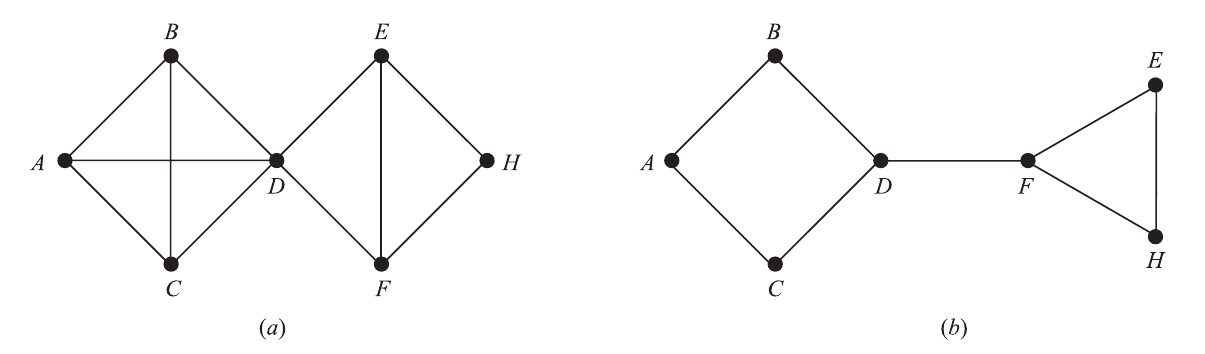
\includegraphics[width=10cm,keepaspectratio=true]{./grafo_8_9.png}
    % grafo_8_9.png: 0x0 pixel, 300dpi, 0.00x0.00 cm, bb=
    \caption{Distancia y diametro}
    \label{fig:md0505}
  \end{figure}
  Por ejemplo, en el grafo \ref{fig:md0505}(a), el diamtero es $3,$ mientras que
  en el (b), el diametro es 4.
\end{frame}

\begin{frame}{Puntos de corte y puentes}
  Sea $G$ un grafo conexo. Un vértice $v$ en $G$ es llamado \emph{punto de
    corte} si $G-v$ es disconexo. Una arista $e$ en $G$ es llamada \emph{puente} si
  $G-e$ es disconexo.

  \begin{figure}[h]
    \centering
    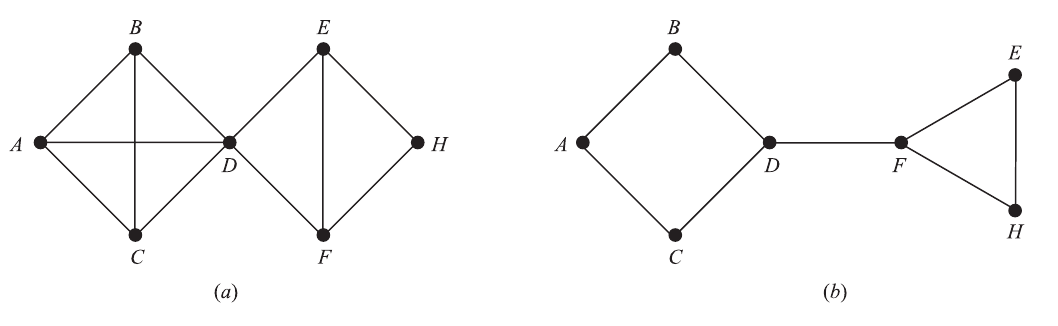
\includegraphics[height=3cm,keepaspectratio=true]{./fig0809.png}
    % fig0809.png: 0x0 pixel, 300dpi, 0.00x0.00 cm, bb=
    \caption{Puntos de corte y puentes}
    \label{fig:0809}
  \end{figure}

\end{frame}

\subsection{Grafos transitables y eulerianos}
\begin{frame}
  \begin{figure}[h!]
    \centering
    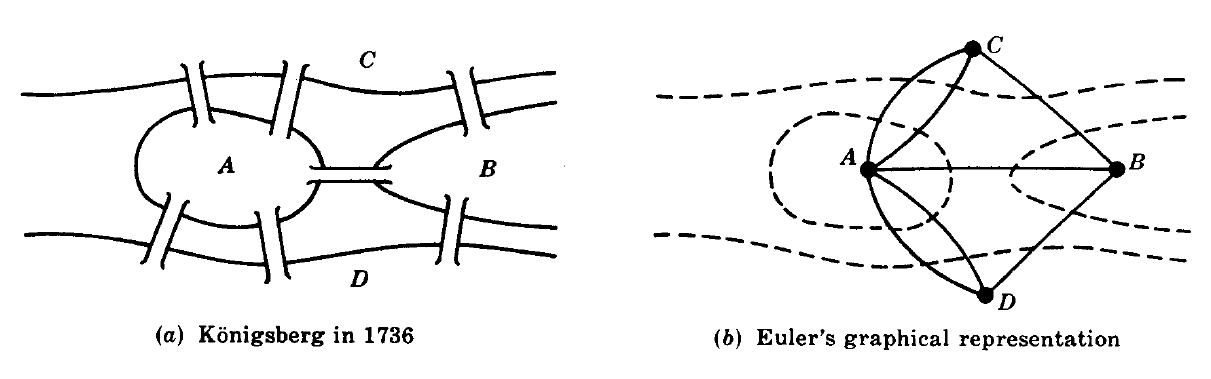
\includegraphics[width=10cm,keepaspectratio=true]{./grafo_8_10.png}
    % grafo_8_10.png: 0x0 pixel, 300dpi, 0.00x0.00 cm, bb=
    \caption{Puentes de K\"onigsberg y su representación}
    \label{fig:md0506}
  \end{figure}
\end{frame}

\begin{frame}
  Un multigrafo es llamado \emph{transitable} si existe un \emph{paseo} (un
  camino dónde todos las aristas son diferentes), que incluye \emph{todos los
    vértices y todas las aristas.}

  Tal paseo será llamado  \emph{paseo transitable}.
  \pause

  \begin{rem}
    De manera equivalente, un paseo transitable es un camino en el que todos los
    vértices se transitan \emph{al menos} una vez,  pero las aristas
    \emph{exactamente} una vez.
  \end{rem}

\end{frame}

\begin{frame}

  \begin{prop}
    Cualquier grafo conexo y finito con exactamente dos vértices impares es
    transitable. Un paseo transitable puede comenzar en alguno de los vértices
    impares y terminar en el otro vértice impar.
  \end{prop}
\end{frame}

\begin{frame}
  Un grafo $G$ es llamado \emph{grafo Euleriano} si existe un \emph{paseo
    transitable cerrado}.

  \pause
  A tal paseo le llamaremos \emph{paseo Euleriano.}
  \pause

  \begin{thm}[Euler]
    Un grafo conexo y finito es Euleriano si y solo si cada vértice tiene grado
    par.
  \end{thm}

\end{frame}

\begin{frame}{Grafos hamiltonianos}
  En la definición de grafos Eulerianos se enfatizó pasar por todas las
  aristas.
  \pause

  Ahora, nos enfocaremos en visitar todos los vértices.
\end{frame}

\begin{frame}
  Un \emph{circuito Hamiltoniano} es un grafo $G$ es un camino cerrado que visita
  cada vértice en $G$ \emph{exactamente} una vez.
  \pause

  Si $G$ admite un circuito Hamiltoniano, entonces $G$ es llamado un \emph{grafo
    Hamiltoniano.}

  \pause
  \begin{rem}
    En la definición de circuito Hamiltoniano, cuando decimos que el camino
    \emph{visita} cada vértice exactamente una vez significa que, aunque el
    vértice inicial tiene que ser el mismo que el final, todos los demás
    vértices intermedios deben ser distintos.
  \end{rem}

\end{frame}

\begin{frame}
  \begin{rem}
    Un {\color{red}paseo Euleriano} atraviesa {\color{red}cada una de las aristas}
    exactamente una vez, pero los vértices se pueden repetir, mientras que un
      {\color{blue}circuito Hamiltoniano} visita {\color{blue}cada uno de los
        vértices} exactamente una vez, pero las aristas pueden repetirse.

  \end{rem}

  \pause

  \begin{thm}
    Sea $G$ un grafo conexo con $n$ vértices. Entonces $G$ es Hamiltoniano si
    $n\geq 3$ y $n \leq \deg(v)$ para cada vértice $v$ en $G.$
  \end{thm}

\end{frame}

\begin{frame}
  \begin{figure}[h!]
    \centering
    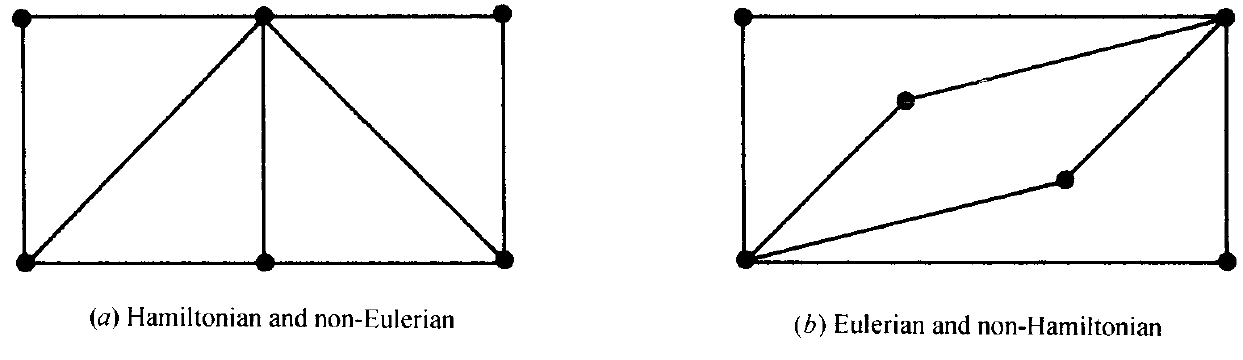
\includegraphics[width=10 cm]{./grafo_8_11.png}
    % grafo_8_11.png: 0x0 pixel, 300dpi, 0.00x0.00 cm, bb=
    \caption{Circuitos Eulerianos y Hamiltonianos}
    \label{fig:md 0506}
  \end{figure}

\end{frame}

\subsection{Matriz de adyacencia}

\begin{frame}
  Supongamos que $G$ es un gráfo con $m$ vértices y que estos han sido
  ordenados:
  $$
    v_{1}, v_{2},...,v_{m}.
  $$

  Entonces, la \emph{matriz de adyacencia} $A=\left( a_{i,j} \right)$ del grafo
  $G$ es la matriz de dimensión $m\times m$ definida por:
  $$a_{i,j}=
    \begin{cases}
      1 & v_{i}\texttt{ es adyacente a }v_{j} \\
      0 & \texttt{en otro caso}
    \end{cases}
  $$
\end{frame}

\begin{frame}
  \begin{figure}[h]
    \centering
    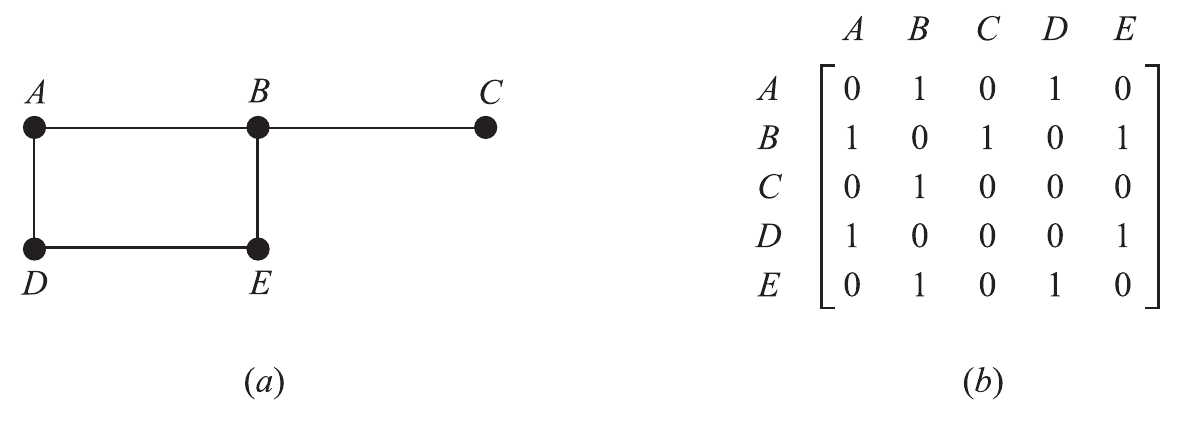
\includegraphics[width=10cm,keepaspectratio=true]{./fig0827.png}
    % fig0827.png: 0x0 pixel, 300dpi, 0.00x0.00 cm, bb=
    \caption{Matriz de adyacencia}
    \label{fig:0827}
  \end{figure}

\end{frame}

\section{Digrafos}

\begin{frame}
  Los \emph{grafos dirigidos} o \emph{digrafos} son grafos en los que las aristas
  tienen una dirección.
\end{frame}

\subsection{Grafos dirigidos}

\begin{frame}
  Un grafo dirigido $G=G(V,E)$ consiste de:
  \begin{enumerate}
    \item Un conjunto $V=V(G)$ cuyos elementos son llamados \emph{vértices};
    \item un conjunto $E=E(G)$ de \emph{pares ordenados} ordenados de vértices
          llamados \emph{arcos} o \emph{aristas dirigidas.}
  \end{enumerate}

\end{frame}

\begin{frame}
  Supongamos que $e=(u,v)$ es un arco en el digrafo $G.$ Entonces, la siguiente
  terminología es usada:
  \begin{itemize}
    \item $e$ comienza en $v$ y termina en $v;$
    \item $u$ es el origen o punto inicial de $e,$ mientras que $v$ es el destino
          o punto final de $e.$
    \item $v$ es un sucesor de $u;$
    \item $u$ es adyacente a $v$ y $v$ es adyacente desde $u.$
  \end{itemize}
  \pause

  Si $u=v,$ $e$ es llamado un \emph{bucle.}
\end{frame}

\begin{frame}
  Si las aristas o los vértices de un digrafo están etiquetas con algún
  tipo de dato, diremos que es un \emph{digrafo etiquetado.}
  \pause

  De manera similar a un grafo, un digrafo será finito si el conjunto de
  vértices y el de aristas es finito.
\end{frame}

\begin{frame}
  \begin{exmp}
    Consideremos el siguiente digrafo.
    \begin{figure}[h]
      \centering
      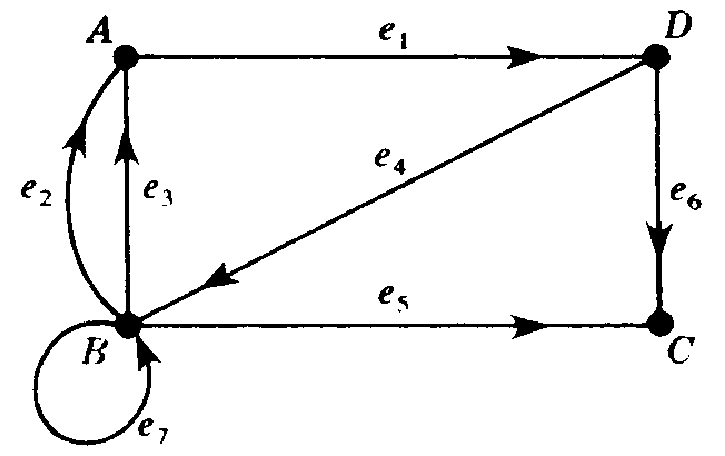
\includegraphics[height=3cm,keepaspectratio=true]{./fig0901a.png}
      % fig0901a.png: 0x0 pixel, 300dpi, 0.00x0.00 cm, bb=
      %\caption{Digrafo}
      \label{fig:0901a}
    \end{figure}
    Las aristas $e_{2}$ y $e_{3}$ son llamados \emph{paralelos,} ya que ambos
    comienzan en $B$ y terminan en $A.$ La arista $e_{7}$ es un \emph{bucle.}
  \end{exmp}

\end{frame}

\begin{frame}
  \begin{exmp}
    \begin{figure}[h]
      \centering
      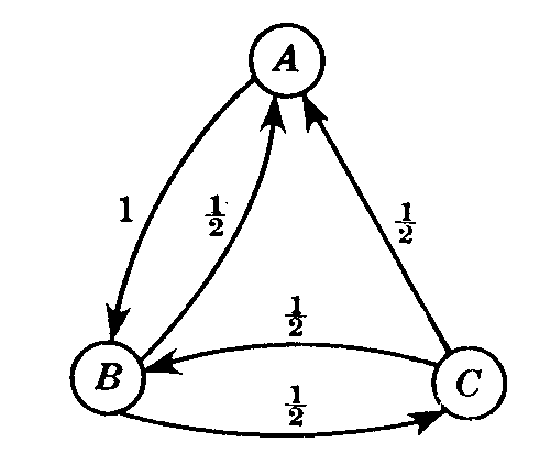
\includegraphics[width=5cm,keepaspectratio=true]{./fig0901b.png}
      % fig0901b.png: 0x0 pixel, 300dpi, 0.00x0.00 cm, bb=
      \caption{Proceso estocástico}
      \label{fig:0901b}
    \end{figure}

  \end{exmp}

\end{frame}

\subsection{Matriz de adyacencia}

\begin{frame}
  Ahora, sólo consideraremos \emph{digrafos simples} $G(V,E)$, es decir, sin
  aristas paralelas. Entonces $E$ es simplemente una relación en $V.$ \pause

  De manera inversa, si $R$ es una relación en $V,$ entonces $G(V,R)$ es un
  digrafo simple.\pause

  En unidades anteriores, ya hemos construido digrafos asociados a relaciones de
  orden parcial, llamados diagramas de Hasse.
\end{frame}

\begin{frame}
  Supongamos que $G$ es un digrafo simple con $m$ vértices, y supongamos que
  los vértices de $G$ han sido ordenados y son llamados $v_{1},
    v_{2},...,v_{m}.$ \pause

  Entonces la \emph{matrix de adyacencia} $A=\left( a_{i,j} \right)$ de $G$ es la
  una matriz de dimensión $m\times m$ definida de la siguiente manera
  $$a_{i,j}=
    \begin{cases}
      1 & \exists e \in E: e=(v_{i}, v_{j}) \\
      0 & \texttt{en otro caso}
    \end{cases}
  $$
\end{frame}

\begin{frame}
  \begin{rem}
    Las matrices de adyacencia de un mismo grafo dependen del orden en que se
    enumeren los vértices. \pause
    Sin embargo, dos matrices de adyacencia de un mismo grafo están
    relacionadas por operaciones elementales: cambiar el orden de columnas y
    renglones.
  \end{rem}

\end{frame}

\begin{frame}
  \begin{exmp}
    Sea $G$ el siguiente digrafo
    \begin{figure}[h]
      \centering
      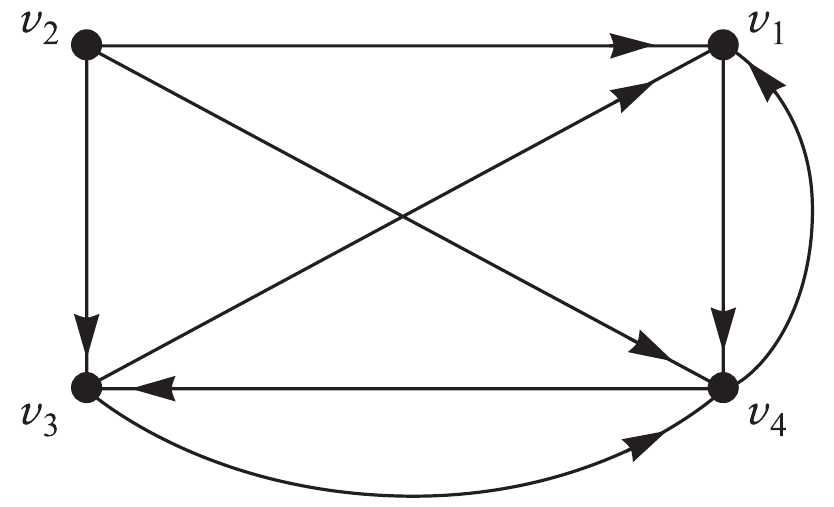
\includegraphics[height=3cm,keepaspectratio=true]{./fig0904a.png}
      % fig0904a.png: 0x0 pixel, 300dpi, 0.00x0.00 cm, bb=
      \caption{Construya su matriz de adyacencia del digrado anterior.}
      \label{fig:0904a}
    \end{figure}

  \end{exmp}

\end{frame}

\begin{frame}
  La matriz identidad $I_{m}=\left( I_{i,j} \right)$ de dimensión $m\times m$
  se define como
  $$I_{i,j}
    \begin{cases}
      1 & i=j       \\
      0 & i \neq j,
    \end{cases}
  $$\pause
  es decir, es matriz cuadrangular con $1's$ en la \emph{diagonal principal}, y
  ceros en cualquier otra entrada.
\end{frame}

\begin{frame}
  \begin{exmp}
    $$I_{2}=
      \begin{pmatrix}
        1 & 0 \\
        0 & 1 \\
      \end{pmatrix}
    $$

    $$I_{3}=
      \begin{pmatrix}
        1 & 0 & 0 \\
        0 & 1 & 0 \\
        0 & 0 & 1
      \end{pmatrix}
    $$
  \end{exmp}

\end{frame}

\begin{frame}
  La propiedad principal de una matriz identidad $I_{m}$ es que es nuestra
  respecto a la multiplicación de matrices\pause, es decir, para cualquier otra
  matriz $A\in M_{n}:$
  $$
    AI_{n}=I_{n}A=A.
  $$
\end{frame}

\begin{frame}
  La potencia $n-$ésima de una matriz $A \in M_{n}$ se define de manera
  recursiva como
  $$
    A^{n}=
    \begin{cases}
      I_{n}    & n=0       \\
      AA^{n-1} & n \in \N.
    \end{cases}
  $$ \pause

  Es decir, $$A^{0}=I, A^{1}=A, A^{2}=AA,...$$
\end{frame}

\begin{frame}
  Definamos $a_{k}(i,j)$ como la entrada en la posición $i,j$ de $A^{k}.$
  \pause

  \begin{prop}
    Sea $A$ la matriz de adyacencia de un grafo $G.$ Entonces $a_{k}(i,j)$ es
    igual al número de caminos de longitud $k$ que van de $v_{i}$ a $v_{j}.$
  \end{prop}

\end{frame}

\begin{frame}{Ejemplo}
  Consideremos nuevamente el grafo
  \begin{figure}[h]
    \centering
    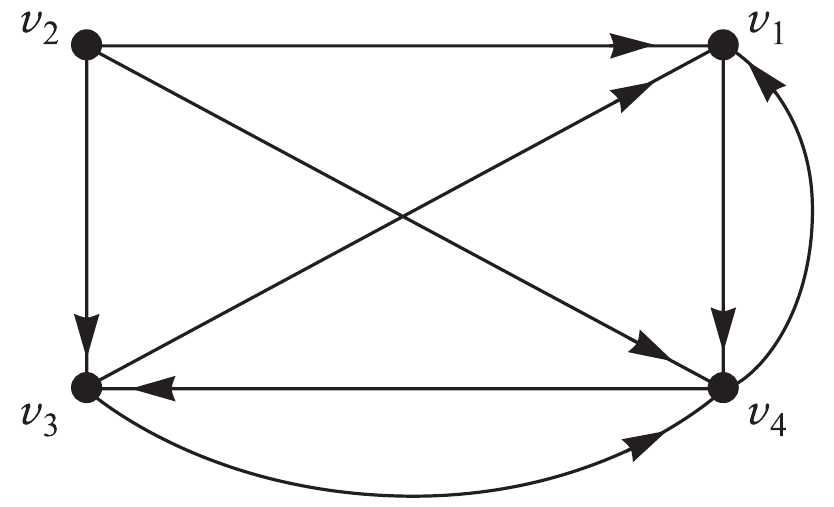
\includegraphics[height=3cm,keepaspectratio=true]{./fig0904a.png}
    % fig0904a.png: 0x0 pixel, 300dpi, 0.00x0.00 cm, bb=
  \end{figure}
\end{frame}

\begin{frame}
  Recordemos que su matriz de adyacencia es
  \begin{equation}
    \label{exmp:adj}
    \tag{AD}
    A= \left(\begin{array}{rrrr}
        0 & 0 & 0 & 1 \\
        1 & 0 & 1 & 1 \\
        1 & 0 & 0 & 1 \\
        1 & 0 & 1 & 0
      \end{array}\right)
  \end{equation}

\end{frame}

\begin{frame}
  Entonces
  $$
    A^{2}= \left(\begin{array}{rrrr}
        1 & 0 & 1 & 0 \\
        2 & 0 & 1 & 2 \\
        1 & 0 & 1 & 1 \\
        1 & 0 & 0 & 2
      \end{array}\right) \;
    A^{3}= \left(\begin{array}{rrrr}
        1 & 0 & 0 & 2 \\
        3 & 0 & 2 & 3 \\
        2 & 0 & 1 & 2 \\
        2 & 0 & 2 & 1
      \end{array}\right) \;
  $$

  $$
    A^{4}= \left(\begin{array}{rrrr}
        2 & 0 & 2 & 1 \\
        5 & 0 & 3 & 5 \\
        3 & 0 & 2 & 3 \\
        3 & 0 & 1 & 4
      \end{array}\right)
  $$
\end{frame}

\begin{frame}
  Observe que $a_{2}(4,1)=1,$ de manera que existe un solo camino de longitud 2
  de $v_{4}$ a $v_{1}.$ De manera similar, como $a_{3}(2,3)=2,$ entonces existen
  dos caminos de longitud $3$ de $v_{2}$ a $v_{3}.$
\end{frame}

\begin{frame}
  \begin{rem}
    Si definimos
    $$B_{r}= \sum_{i=1}^{r}A^{i},$$
    entonces la entrada $i,j$ de esta matriz nos indicará el número de caminos
    de longitud a lo más $r$ de $v_{i}$ a $v_{j}.$
  \end{rem}
\end{frame}

\begin{frame}
  En nuestro ejemplo, considerando $A$ dado por \eqref{exmp:adj}, tenemos que
  \begin{equation}
    \label{B4}
    B_{4}=
    \left(\begin{array}{rrrr}
        4  & 0 & 3 & 4  \\
        11 & 0 & 7 & 11 \\
        7  & 0 & 4 & 7  \\
        7  & 0 & 4 & 7
      \end{array}\right)
  \end{equation}
  \pause

  ?`Existe alguna manera de llegar al vertice $v_{2}$ desde el vértice $v_{1}$,
  sin importar la longitud del camino?
\end{frame}

\subsection{Matriz de accesibilidad}

\begin{frame}
  Sea $G=G(V,E)$ un grafo simple dirigido con $m$ vértices $v_{1},...,v_{m}.$
  La \emph{matriz de accesibilidad} de $G$ es la matriz $m-$cuadrangular
  $P=\left( p_{ij} \right)$ definida de la siguiente manera:
  $$p_{ij}=
    \begin{cases}
      1 & \texttt{existe un camino de }v_{i}\texttt{ a }v_{j} \\
      0 & \texttt{en otro caso}
    \end{cases}
  $$
\end{frame}

\begin{frame}
  \begin{prop}
    Sea $A$ la matriz de adyacencia de un grafo $G$ con $m$ vértices. Entonces
    la matriz de accesibilidad y
    \begin{equation}
      \label{Bm}
      B_{m}=\sum_{i=1}^{m}A^{i}
    \end{equation}
    tienen exactamente las mismas entradas no nulas.
  \end{prop}

\end{frame}

\begin{frame}
  \begin{defn}
    Un digrafo es \emph{fuertemente conexo} si para cualquier par de vértices
    $u,v$ existe al menos un camino de $u$ a $v$ y otro de $v$ a $u.$
  \end{defn}

\end{frame}

\begin{frame}
  \begin{prop}
    Sea $A\in M_{m}$ la matriz de adyacencia de un grafo $G.$ Entonces, las
    siguientes proposiciones son equivalentes:
    \begin{enumerate}
      \item $G$ es fuertemente conexo;
      \item la matriz de accesibilidad $P$ no tiene entradas nulas;
      \item la matriz $B_{m},$ dada por \eqref{Bm}, no tiene entradas nulas.
    \end{enumerate}

  \end{prop}

\end{frame}

\begin{frame}
  \begin{exmp}
    \label{lip:exmp:0908}
    Para encontrar la matriz de accesibilidad asociada a la matriz de adyacencia
    $A,$ dada por \eqref{exmp:adj}, basta sustitur las entradas no nulas en la
    matriz $B_{4},$ dada por \eqref{B4}, por $1's:$
    $$
      P=
      \left(\begin{array}{rrrr}
          1 & 0 & 1 & 1 \\
          1 & 0 & 1 & 1 \\
          1 & 0 & 1 & 1 \\
          1 & 0 & 1 & 1
        \end{array}\right)
    $$
  \end{exmp}

\end{frame}

\end{document}
